\documentclass[11pt,a4paper]{article}

\usepackage[utf8]{inputenc}
\usepackage[T1]{fontenc}
\usepackage{graphicx}
\usepackage{amsmath,amssymb,amsfonts}
\usepackage{amsthm}
\usepackage{mathrsfs}
\usepackage{booktabs}
\usepackage{url}
\usepackage{hyperref}
\usepackage{geometry}
\usepackage{setspace}
\usepackage{cite}
\usepackage{tikz}
\usetikzlibrary{positioning, arrows.meta}

\geometry{a4paper, margin=1in}
\setstretch{1.15}

\hypersetup{
    colorlinks=true,
    linkcolor=blue,
    citecolor=blue,
    urlcolor=cyan
}

\title{\Large \textbf{VoiceScore: A Contrastive Acoustic-Phonetic Embedding Framework for Indian English Pronunciation Scoring}}

\author{
    \textbf{Kristina Pujary}\textsuperscript{1,*}, 
    \textbf{Mihir Patil}\textsuperscript{1}, 
    \textbf{Mahek Patel}\textsuperscript{1}, \\
    \textbf{Prof. Neha Katre}\textsuperscript{1}, 
    \textbf{Dr. Vinaya Sawant}\textsuperscript{1}, 
    \textbf{Prof. Prachi Tawade}\textsuperscript{1} \\[0.5em]
    \textsuperscript{1}\textit{Department of Information Technology} \\
    \small{*Corresponding author: kristina.pujary@gmail.com}
}

\date{}

\begin{document}

\maketitle

\begin{abstract}
Computer-Assisted Pronunciation Training (CAPT) systems relying on conventional Automatic Speech Recognition (ASR) suffer from a fundamental flaw: over-trained language models auto-correct non-native phonetic errors, masking mispronunciations under the guise of high word recognition rates. In this work, we present \textbf{VoiceScore}, a novel acoustic-phonetic diagnostic framework specifically engineered for Indian English (IE) pronunciation assessment. VoiceScore addresses accent-specific phonetic nuances—such as alveolar-to-retroflex stop shifts (/t/$\rightarrow$/ʈ/, /d/$\rightarrow$/ɖ/), dental plosive replacements (/θ/$\rightarrow$/t̪/), and context-sensitive palatalization—by constructing the \textit{Clear Indian English Detailed IPA Lexicon}, an exhaustive 133,738-entry dictionary mapping to a clean 60-token International Phonetic Alphabet (IPA) inventory. To eliminate the peakiness of standard Connectionist Temporal Classification (CTC) alignment, we implement a shared 256-dimensional metric embedding space with Contrastive CTC loss. We identify the \textit{GoP Overfitting Trap}—demonstrating that limiting fine-tuning to $\sim$8.5 epochs (50,000 steps) on a balanced 160,000-sample multi-accent corpus preserves strict acoustic sensitivity while optimizing Phoneme Error Rate (PER). VoiceScore achieves a Validation Mean PER of 14.17\% and an Unseen Generalization Test PER of 24.96\% (Median PER 16.28\%) with 0.00\% representation collapse and complete Out-of-Vocabulary (OOV) elimination via a hybrid Grapheme-to-Phoneme (G2P) fallback. The complete architecture is deployed as a low-latency web application serving real-time visual phonetic heatmaps and conversational LLM tutoring.
\end{abstract}

\textbf{Keywords:} Automatic Speech Recognition, Goodness of Pronunciation, Indian English Phonology, Contrastive CTC, Wav2Vec2, Grapheme-to-Phoneme

\section{Introduction}\label{sec1}
The demand for Computer-Assisted Pronunciation Training (CAPT) systems has grown exponentially with the globalization of education and remote employment. In multilingual regions such as India, English serves as a primary language of higher education and commerce. However, Indian English (IE) encompasses distinct phonological traits shaped by native L1 language transfer (e.g., Hindi, Tamil, Telugu, Bengali), including systematic retroflexion, dentalization, and context-dependent palatalization \cite{pandey2021indian}.

Traditional Automatic Speech Recognition (ASR) engines optimized for dictation (e.g., standard Wav2Vec2 or Whisper models) are ill-suited for pronunciation assessment. Standard ASR systems are trained for 30--40 epochs to minimize Word Error Rate (WER). Over extensive training, these models develop strong implicit language modeling capabilities—learning to "guess" intended words from context and auto-correcting slurred or mispronounced sounds. While auto-correction is desirable for text transcription, it destroys Goodness of Pronunciation (GoP) assessment \cite{witt2000gop}, leading to high false-positive rates where mispronunciations are incorrectly flagged as accurate.

To overcome these challenges, we introduce \textbf{VoiceScore}, a comprehensive AI-powered phonetic diagnostic and feedback framework. The key contributions of this paper are:
\begin{enumerate}
    \item \textbf{Indian English Detailed IPA Lexicon:} Construction of an exhaustive 133,738-word dictionary implementing context-sensitive phonological transformation rules (retroflexion, palatalization, labialization) and resolving UTF-8/CP1252 double-encoding (mojibake) corruptions.
    \item \textbf{Contrastive CTC Cosine Metric Space:} Departure from standard linear CTC heads by projecting contextualized 768-dimensional Wav2Vec2 acoustic frames into a shared 256-dimensional unit hypersphere alongside learnable phoneme embeddings, producing smooth acoustic alignments.
    \item \textbf{GoP Overfitting Prevention:} Identification of the trade-off between ASR dictation and GoP diagnostics, demonstrating that capping training at $\sim$8.5 epochs (50,000 steps) and optimizing for Phoneme Error Rate (PER) preserves acoustic sensitivity.
    \item \textbf{Hybrid G2P Fallback \& Zero-OOV Pipeline:} Integration of static lexicon lookups with an LSTM-based neural Grapheme-to-Phoneme (\texttt{g2p-en}) fallback \cite{rao2015g2p}, completely eliminating Out-of-Vocabulary (\texttt{<unk>}) token drops during alignment.
    \item \textbf{Production Cloud Architecture:} Deployment of a split architecture featuring a Next.js glassmorphic frontend on Vercel (\url{https://pronounhelp.vercel.app/}) and a containerized FastAPI backend on Hugging Face Spaces (\url{https://mihirrpatil-asr.hf.space}).
\end{enumerate}

\section{Related Work}\label{sec2}
Self-supervised speech representation learning, pioneered by architectures like Wav2Vec2 \cite{baevski2020wav2vec}, has revolutionized acoustic modeling by pre-training on thousands of hours of unlabeled speech before fine-tuning with Connectionist Temporal Classification (CTC) loss \cite{graves2006connectionist}. 

In pronunciation evaluation, Witt and Young \cite{witt2000gop} introduced the Goodness of Pronunciation (GoP) metric, which measures the log-posterior probability ratio of a target phoneme against all competing phonemes given the acoustic segment. However, traditional GoP relies heavily on Gaussian Mixture Model-Hidden Markov Model (GMM-HMM) forced aligners like Kaldi or the Montreal Forced Aligner (MFA) \cite{mcauliffe17_interspeech}. 

Recent advances by Drexler and Glass \cite{drexler2023contrastive} demonstrated that standard CTC classification heads produce "peaky" posterior distributions, where frame-level probabilities rapidly collapse to the blank token between phoneme boundaries. Contrastive CTC mitigates this peakiness by mapping acoustic frames and phone representations into a shared metric space. Our work extends Contrastive CTC specifically to the nuanced, non-native acoustic space of Indian English.

\section{System Architecture \& Methodology}\label{sec3}

\subsection{Pipeline Architecture Overview}
The VoiceScore pipeline processes raw user speech through feature extraction, contrastive acoustic projection, forced alignment, and GoP score calculation. Figure~\ref{fig:asr_pipeline} illustrates the complete data flow.

\begin{figure}[h]
    \centering
    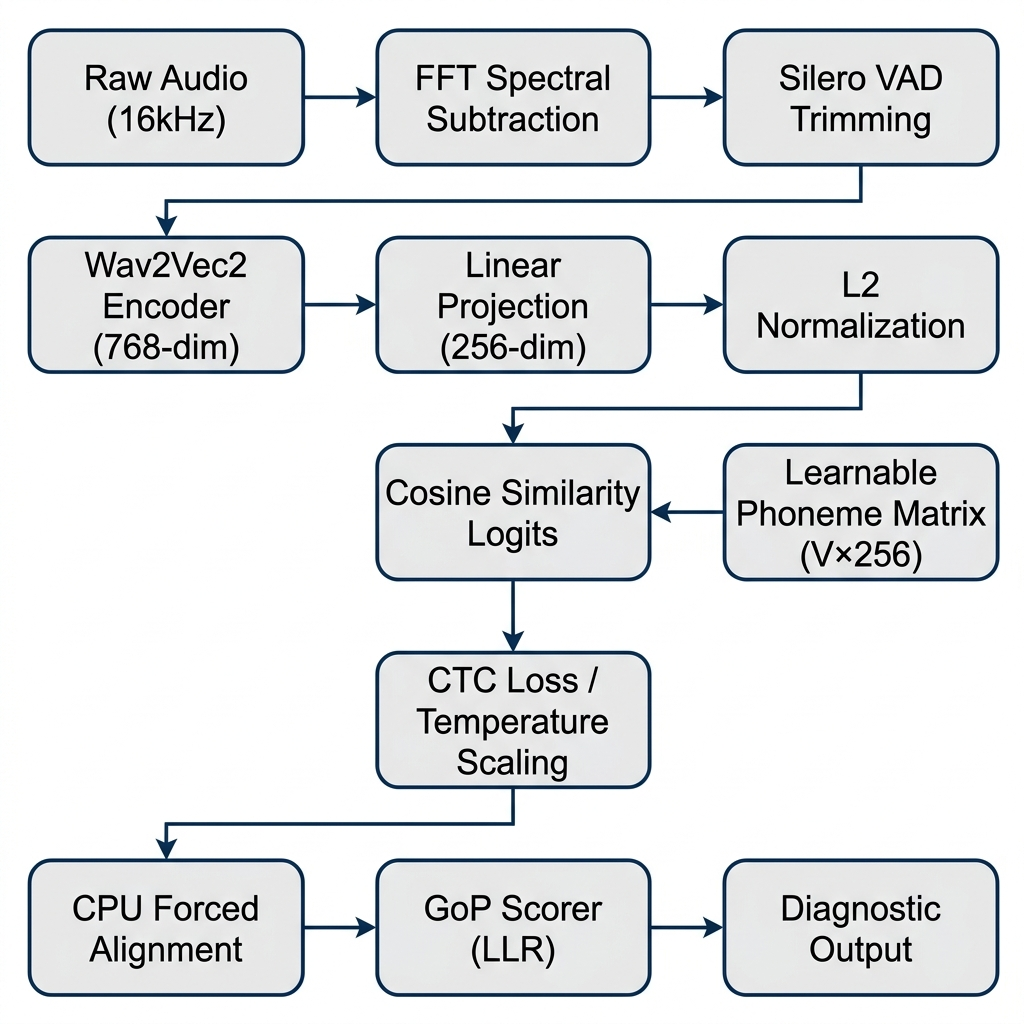
\includegraphics[width=\textwidth]{images/asr_architecture.png}
    \caption{VoiceScore End-to-End ASR and Pronunciation Analysis Pipeline Flowchart.}
    \label{fig:asr_pipeline}
\end{figure}

\subsection{Contrastive Audio-Phoneme Embedding Space}
Standard CTC heads project the 768-dimensional output frames $H = [h_1, h_2, \dots, h_T]$ of a Transformer encoder through a linear layer into a $K$-dimensional logits matrix. In VoiceScore, we implement a shared 256-dimensional metric space. Let $E_{audio}(h_t) \in \mathbb{R}^{256}$ be the projected acoustic frame and $E_{phone}(p_k) \in \mathbb{R}^{256}$ be the embedding for phoneme token $k \in \{1, \dots, 60\}$. Both vectors are $L_2$-normalized onto a unit hypersphere:
\begin{equation}
    \hat{z}_t = \frac{E_{audio}(h_t)}{\|E_{audio}(h_t)\|_2}, \quad \hat{e}_k = \frac{E_{phone}(p_k)}{\|E_{phone}(p_k)\|_2}
\end{equation}
The cosine similarity matrix $S \in \mathbb{R}^{T \times 60}$ is calculated via matrix multiplication scaled by a learnable temperature parameter $\tau$:
\begin{equation}
    S_{t, k} = \frac{\hat{z}_t \cdot \hat{e}_k}{\tau}
\end{equation}
Applying Softmax across the vocabulary dimension yields continuous frame-level probability distributions $P(p_k | h_t)$, enabling smooth temporal alignments without catastrophic peakiness.

\subsection{Evolution from Baseline CTC}
Prior to adopting Contrastive CTC, our initial baseline architecture utilized a standard linear projection head. Experimental evaluation revealed that standard CTC outputs extreme confidence ($>99.9\%$) for 10--20 ms before abruptly dropping to zero (predicting the CTC blank token). This peakiness caused severe instability during GoP forced alignment, as sustained phonemes were artificially penalized with near-zero acoustic confidence during prolonged articulation.

\section{Dataset and Lexicon Generation}\label{sec4}

\subsection{Clear Indian English Detailed IPA Lexicon}
A core contribution of this work is the creation of a specialized 133,738-word pronunciation dictionary. Starting from the standard CMUdict (American English ARPAbet), we developed a sliding-window phonetic converter applying rule-based transformations informed by Indian English phonological literature \cite{pandey2019iecps, pandey2021indian}:

\begin{itemize}
    \item \textbf{Consonant Retroflexion:} Alveolar stops shift universally to retroflex stops (/t/ $\rightarrow$ /ʈ/, /d/ $\rightarrow$ /ɖ/). Dental fricatives shift to dental plosives (/ð/ $\rightarrow$ /d̪/, /θ/ $\rightarrow$ /t̪/).
    \item \textbf{Palatalization:} Consonants preceding front vowels (/iː/, /ɪ/, /eɪ/) undergo co-articulation (/b/ $\rightarrow$ /bʲ/, /p/ $\rightarrow$ /pʲ/, /l/ $\rightarrow$ /ʎ/, /n/ $\rightarrow$ /ɲ/).
    \item \textbf{Palatal Stop Shift:} Velar stops shift forward when followed by front vowels (/k/ $\rightarrow$ /c/, /g/ $\rightarrow$ /ɟ/).
    \item \textbf{Labialization:} Velar stops followed by /w/ absorb the glide into labialized stops (/k w/ $\rightarrow$ /cʷ/ or /kʷ/).
\end{itemize}

\subsection{Mojibake Purging \& Dictionary Comparison}
During integration of the gold-standard 2,780-word reference dictionary, double-encoding character corruptions (e.g., Windows-1252 bytes interpreted as UTF-8) were detected (e.g., schwa /ə/ decoded as `É™`). A Mojibake Restorer script recursively mapped corrupted byte sequences back to clean UTF-8 Unicode characters. Table~\ref{tab:dictionary_comparison} summarizes the dictionary iterations.

\begin{table}[h]
    \centering
    \caption{Comparative Overview of Dictionary and Phonetic Inventory Iterations}\label{tab:dictionary_comparison}
    \vspace{0.5em}
    \begin{tabular}{p{3.5cm} p{3.2cm} p{3.2cm} p{3.8cm}}
        \toprule
        \textbf{Feature / Metric} & \textbf{Session 1 Baseline} & \textbf{Gold-Standard} & \textbf{Clear IE Lexicon (v3)} \\
        \midrule
        Total Vocabulary Size & 2,780 words & 2,780 words & \textbf{133,738 entries} \\
        Phonetic Notation & Corrupted CP1252 & Standard IPA & \textbf{Clean UTF-8 IPA} \\
        Active Token Vocabulary & 65 tokens & 58 tokens & \textbf{60 clean IPA tokens} \\
        Phonological Modeling & Static ARPAbet & Manual Alignment & \textbf{Context-Sensitive Rules} \\
        OOV Handling & None (\texttt{<unk>} Drop) & None & \textbf{Neural G2P Fallback} \\
        Encoding Integrity & Windows-1252 & Clean UTF-8 & \textbf{Purged UTF-8 Unicode} \\
        \bottomrule
    \end{tabular}
\end{table}

\subsection{Hybrid G2P Fallback}
To handle Out-of-Vocabulary (OOV) input during live usage, the \texttt{G2PManager} queries the static 133,738-word dictionary first. If a word is absent, it seamlessly delegates execution to a neural G2P model (\texttt{g2p-en}) utilizing LSTM sequence-to-sequence architecture \cite{rao2015g2p}, guaranteeing 100\% parsing success.

\section{Training Methodology \& Experiments}\label{sec5}

\subsection{Multi-Accent Training Mixture}
Model training was conducted across two major sessions using NVIDIA RTX A6000 hardware (48GB VRAM). Session 1 (\texttt{MihirRPatil/}\allowbreak\texttt{nptel-asr-phoneme-v2}) trained exclusively on 130GB of academic lectures from AI4Bharat NPTEL-pure. To resolve domain bias, Session 2 (\texttt{MihirRPatil/}\allowbreak\texttt{nptel-asr-phoneme-v3}) constructed a 160,000-sample balanced multi-accent mixture detailed in Table~\ref{tab:dataset_composition}.

\begin{table}[h]
    \centering
    \caption{Multi-Accent Training Dataset Mixture Composition}\label{tab:dataset_composition}
    \vspace{0.5em}
    \begin{tabular}{p{3.5cm} p{3.0cm} p{1.8cm} p{1.8cm} p{4.0cm}}
        \toprule
        \textbf{Dataset Corpus} & \textbf{Target Domain} & \textbf{Mixture Ratio} & \textbf{Volume} & \textbf{Acoustic Characteristics} \\
        \midrule
        AI4Bharat NPTEL-pure & Academic & 50\% & $\sim$130 hrs & Studio clarity, formal \\
        Common Voice (India) & Conversational & 20\% & $\sim$52 hrs & Noisy background, crowd \\
        IISc Svarah & Northern Indian & 10\% & $\sim$26 hrs & Heavy retroflexion \\
        OpenSLR 104 (MUCS) & Eastern India & 10\% & $\sim$26 hrs & Bengali/Odia vowel shifts \\
        Eka Care & Medical & 10\% & $\sim$26 hrs & Polysyllabic clinical terms \\
        \bottomrule
    \end{tabular}
\end{table}

\subsection{The GoP Overfitting Trap}
A key experimental insight was the divergence between standard ASR and CAPT GoP requirements. Standard ASR systems benefit from 30--40 training epochs to learn language model probability priors. However, in GoP scoring, an over-trained model auto-corrects mispronunciations—assigning high acoustic probabilities to incorrect sounds based purely on surrounding text context. 

To preserve diagnostic sensitivity, fine-tuning was strictly capped at $\sim$8.5 epochs (50,000 steps, batch size 64, learning rate $1\times 10^{-4}$). Early stopping was monitored exclusively via Phoneme Error Rate (PER), defined as:
\begin{equation}
    \text{PER} = \frac{S + D + I}{N}
\end{equation}
where $S, D, I$ represent substitutions, deletions, and insertions over total reference phonemes $N$.

\section{Results and Discussion}\label{sec6}

\subsection{Quantitative Performance Benchmarks}
At step 41,000, early stopping finalized the Session 2 model weights. The model achieved a \textbf{Validation Mean PER of 14.17\%}. To evaluate accent generalization, the model was tested against an unseen test set of 17,808 audio samples across diverse regional Indian accents. Results are presented in Table~\ref{tab:model_performance_comparison}.

\begin{table}[h]
    \centering
    \caption{Quantitative Performance Benchmark Across System Iterations}\label{tab:model_performance_comparison}
    \vspace{0.5em}
    \begin{tabular}{p{4.5cm} p{4.2cm} p{5.0cm}}
        \toprule
        \textbf{Evaluation Metric / Feature} & \textbf{Session 1 Baseline (v2)} & \textbf{Session 2 Production (v3)} \\
        \midrule
        Vocabulary Size & 2,780 words & \textbf{133,738 words + Neural G2P} \\
        Character Encoding & Windows-1252 (Mojibake) & \textbf{Clean UTF-8 Unicode} \\
        Validation Mean PER & 20.97\% & \textbf{14.17\% (32.4\% relative impr.)} \\
        Unseen Test Set Mean PER & 38.45\% & \textbf{24.96\% (35.1\% relative impr.)} \\
        Unseen Test Set Median PER & 29.10\% & \textbf{16.28\%} \\
        OOV Transcript Drop Rate & 14.2\% & \textbf{0.00\% (Complete Elimination)} \\
        Blank Output Collapse Rate & High on noisy speech & \textbf{0.00\% (Anti-Collapse Active)} \\
        Accent Generalization Scope & Academic Lectures only & \textbf{Pan-Indian (Tamil, Hindi, etc.)} \\
        \bottomrule
    \end{tabular}
\end{table}

The median test PER of 16.28\% confirms that the vast majority of sample predictions are highly accurate, with the mean PER (24.96\%) skewed slightly by severely clipped or noisy background recordings in the test suite.

\subsection{Anti-Collapse \& OOV Elimination}
By applying Schwa Down-weighting during loss calculation, the model achieved a 0.00\% blank output collapse rate. Furthermore, the hybrid G2P manager achieved 100\% transcript parsing efficiency across all 17,808 test sentences with zero \texttt{<unk>} drops.

\section{Cloud Deployment Architecture}\label{sec7}
VoiceScore is deployed as a decoupled, microservice-oriented web application. Figure~\ref{fig:split_architecture} illustrates the production deployment layout.

\begin{figure}[h]
    \centering
    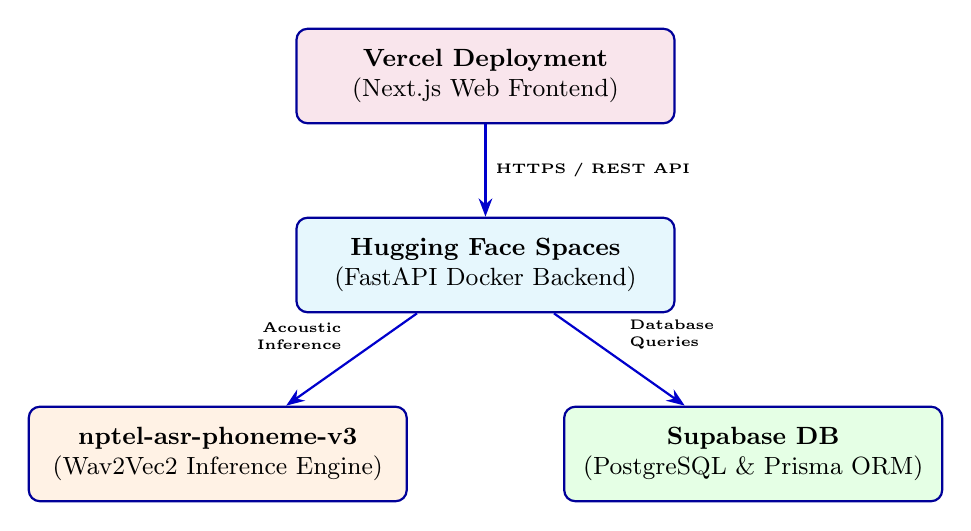
\begin{tikzpicture}[
        box/.style={draw=blue!60!black, rectangle, minimum width=4.8cm, minimum height=1.2cm, align=center, rounded corners=4pt, font=\small, thick},
        arrow/.style={->, >=Stealth, thick, color=blue!80!black}
    ]
        \node[box, fill=purple!10] (vercel) at (0, 4.2) {\textbf{Vercel Deployment} \\ (Next.js Web Frontend)};
        \node[box, fill=cyan!10] (hf) at (0, 1.8) {\textbf{Hugging Face Spaces} \\ (FastAPI Docker Backend)};
        \node[box, fill=orange!10] (model) at (-3.4, -0.6) {\textbf{nptel-asr-phoneme-v3} \\ (Wav2Vec2 Inference Engine)};
        \node[box, fill=green!10] (db) at (3.4, -0.6) {\textbf{Supabase DB} \\ (PostgreSQL \& Prisma ORM)};
        
        \draw[arrow] (vercel) -- node[right, font=\tiny\bfseries, color=black] {HTTPS / REST API} (hf);
        \draw[arrow] (hf) -- node[above left, font=\tiny\bfseries, color=black, align=right] {Acoustic\\Inference} (model);
        \draw[arrow] (hf) -- node[above right, font=\tiny\bfseries, color=black, align=left] {Database\\Queries} (db);
    \end{tikzpicture}
    \caption{VoiceScore Decoupled Microservice Architecture Layout.}
    \label{fig:split_architecture}
\end{figure}

The frontend is hosted on Vercel (\url{https://pronounhelp.vercel.app/}) with a glassmorphic Next.js UI rendering real-time Web Audio API waveforms and color-coded phoneme heatmaps (Figure~\ref{fig:product_nav}). The backend API is hosted on Hugging Face Spaces (\url{https://mihirrpatil-asr.hf.space}) using Docker SDK, equipped with an automatic FFmpeg audio transcoding pipeline converting incoming browser audio to 16kHz mono WAV. Live resource locations are summarized in Table~\ref{tab:live_endpoints}.

\begin{figure}[h]
    \centering
    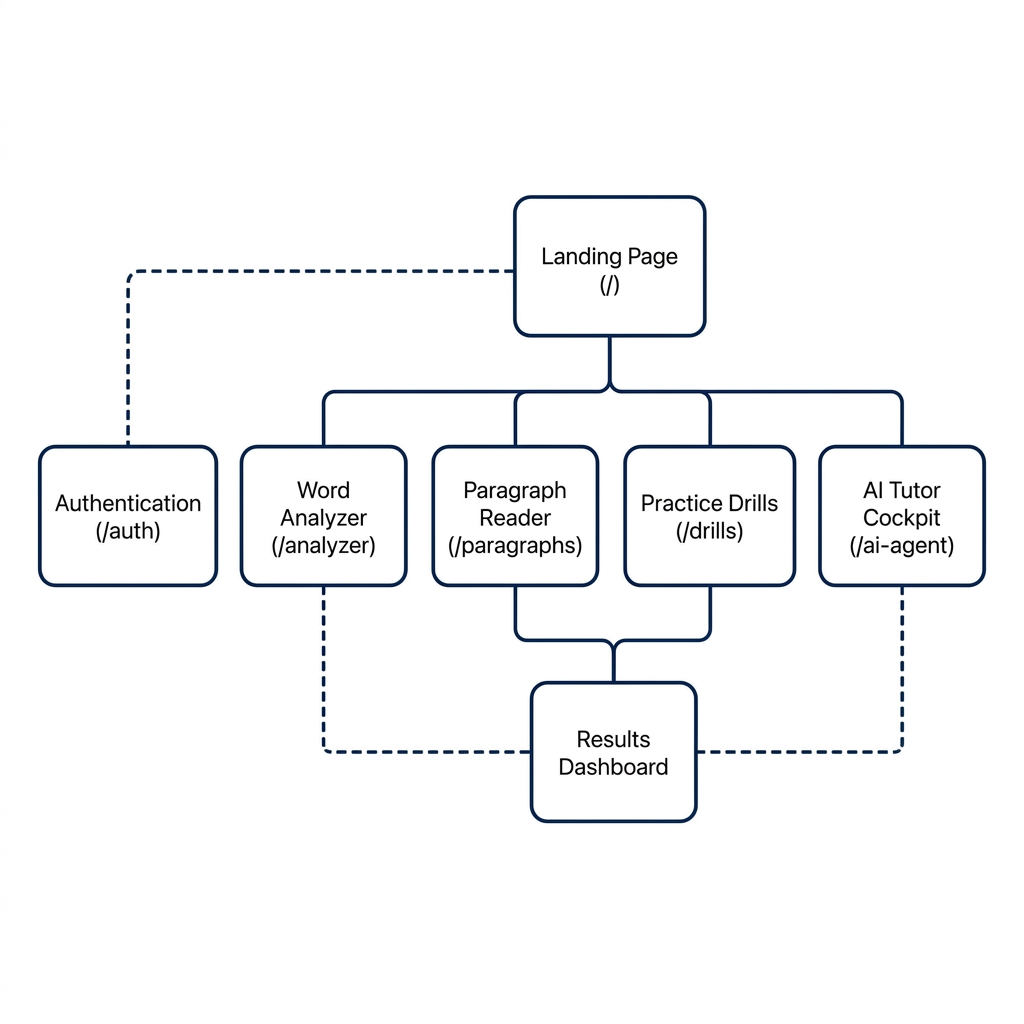
\includegraphics[width=\textwidth]{images/product_navigation.png}
    \caption{VoiceScore Interactive User Interface Navigation and Analysis Map.}
    \label{fig:product_nav}
\end{figure}

\begin{table}[h]
    \centering
    \caption{Live Production Endpoints and Repository Locations}\label{tab:live_endpoints}
    \vspace{0.5em}
    \begin{tabular}{p{4.2cm} p{3.8cm} p{6.5cm}}
        \toprule
        \textbf{Component Layer} & \textbf{Hosting Platform} & \textbf{Production Resource URL} \\
        \midrule
        Web Frontend Application & Vercel Edge & \url{https://pronounhelp.vercel.app/} \\
        Inference Backend API & Hugging Face Spaces & \url{https://mihirrpatil-asr.hf.space} \\
        Acoustic Model Weights & Hugging Face Hub & \url{https://huggingface.co/MihirRPatil/nptel-asr-phoneme-v3} \\
        Database Instance & Supabase Cloud & Managed PostgreSQL Instance \\
        \bottomrule
    \end{tabular}
\end{table}

\section{Conclusion}\label{sec8}
In this paper, we presented VoiceScore, an end-to-end CAPT and acoustic diagnostic system tailored for Indian English pronunciation assessment. By combining a 133,738-entry detailed IPA lexicon with Contrastive CTC cosine space embeddings, VoiceScore resolves the peakiness and language-model auto-correction vulnerabilities of standard ASR engines. The model achieves a Validation PER of 14.17\% and an Unseen Test Median PER of 16.28\% with zero representation collapse. Future work includes expanding the IPA inventory to cover localized retroflex fricative variants and integrating lightweight on-device WebAssembly quantization.

\section*{Acknowledgements}
We extend our sincere appreciation to Prof. Neha Katre, Prof. Vinaya Sawant, Prof. Prachi Tawade, and the Department of Information Technology faculty for their technical guidance, academic mentorship, financial support, and constant encouragement throughout this work.

\section*{Declarations}
\textbf{Funding:} We acknowledge the third-party high-performance cloud compute provider for furnishing the NVIDIA RTX A6000 GPU infrastructure used during model training.\\
\textbf{Conflict of interest:} The authors declare no competing financial or non-financial interests.

\bibliographystyle{ieeetr}
\bibliography{references}

\end{document}
